\vspace{-0.05in}
\section{Experiments}
\label{sec:experiments}
\vspace{-0.05in}
%Unlike regular crowdsourcing, there is no publicly available platform for running real-world spatial crowdsourcing campaigns. With platforms such as Amazon Mechanical Turk, workers do not perform spatial crowdsourcing tasks. For this reason, we simulated various spatial crowdsourcing campaigns on an Inter(R) Core(TM)2 Duo 3.16GHz PC with 4GB memory running Microsoft Windows 7.

\subsection{Dataset}
\label{subsec:dataset}
\vspace{-0.05in}
%Due to its commercial value, real-life SC systems such as Uber and TaskRabbit do not make their datasets available to public. 
We evaluate our algorithms using real check-in data in Foursquare and Gowalla and convert them to spatial tasks and workers in our system. We consider check-ins as a spatial task performed at the location the check-in happened. For each location, we consider all check-ins within a two hours duration. For each task, we set the release time and deadline to the first and last check-in time within the two hours duration. We consider each user as a spatial worker with start and end times equal to the user's first and last check-in during a day. We select the initial location of a worker as a random point within the bounding box of all checked-in locations of the corresponding user. We also measure the travel time with the Euclidean distance between two points divided by an average speed of $60 km/h$. We use the data from 5 metropolitan areas: New York, Los Angeles, Paris, London \& Beijing. \cref{tab:flickr_stats} shows the total number of tasks (and workers) for each city.

\begin{table}[h]
\begin{center}
\begin{tabular}{| l || c | c || c | c |} \hline
			& \multicolumn{2}{c||}{Gowalla}		&\multicolumn{2}{c|}{Foursquare}		\\ \hline
			&	\# Tasks	&	\#  Workers		&	\#  Tasks	&	\#  Workers		\\ \hline
Los Angeles	&	197,353		&		4,126		&	185,061		&		9,136		\\ \hline
New York	&	118,406		&		3,987		&	577,124		& 		17,367		\\ \hline
London		& 	60,180		&		2,294		&	186,755		&		9,711		\\ \hline
Paris		&	18,932		&		1,829		&	105,998		&		6,095		\\ \hline
Beijing		&	3,638		&		699			&	21,013		&		1,075		\\ \hline
\end{tabular}
\caption{\small{Number of tasks/worker for each city in real dataset}}
\vspace{-0.2in}
\label{tab:flickr_stats}
\end{center}
\end{table}

We also generate a synthetic datasets with realistic streaming workload using \cite{To15}. To generate a workload suitable for SC systems, we modeled three different sets of parameters:

\noindent \textbf{Temporal Parameters:} We assume workers and tasks arrive following Poisson processes. In our experiments, the default Poisson arrival rates for tasks and workers are \boldmath$\mu_t = 20/min$ and $\mu_w = 3/min$, respectively. Subsequently, the duration of the tasks and workers were randomly sampled from closed range of \boldmath{$\left[1,4 \right]$} \textbf{hours} and $\left[1,8 \right]$ \textbf{hours}, respectively.

\noindent \textbf{Spatial Parameters:} \cref{fig:la_gowalla} shows the spatial distribution of tasks from our real-world dataset in Los Angeles. As depicted, the tasks are not uniformly distributed in space. The spatial distribution is rather skewed, meaning that the density of the tasks at certain areas is higher. To model the same behavior with our synthetic workloads, we created 6 two dimensional Gaussian clusters with randomly selected means and standard deviations. Eighty percent of the tasks are sampled within the clusters and the rest are uniformly distributed.

\noindent \textbf{Static Parameters:} In addition to the spatiotemporal parameters, we consider two other parameters. The default \emph{workload size} of each experiment is \textbf{50K tasks}. The task arrival rate and the number of tasks determine the duration of the simulation. Based on the duration of the simulation and the workers' arrival rate, the total number of workers may vary. The maximum number of tasks a worker can perform, i.e., $w_{max}$, is a uniformly random number from the closed interval \boldmath$\left[8,12 \right]$.

\begin{figure}[h]
	\centering
	\includegraphics[scale=0.35]{figures/la_flickr.jpg}
	\caption{Spatial Distribution of Tasks in Gowalla}\label{fig:la_gowalla}
\end{figure}

\vspace{-0.05in}
\subsection{Experimental Methodology}
\label{subsec:exp_setup}
\vspace{-0.05in}
\subsubsection{Algorithms}
We compared the results of our framework(\textbf{AUC}) with three other approaches: \textbf{NN} (i.e., nearest neighbor) as a scheduling-oblivious-matching (SOM) approach, \textbf{BCHD} (i.e., batched) and \textbf{MONO} (i.e., online monolithic-SC).

We explained that the SOM approach is when the tasks are assigned to workers without considering the workers' schedules. In other words, the server assigns tasks to workers based on some heuristic and once the task is assigned to a worker, the worker attempts to add the task to its schedule. If it succeeds then the task gets completed and otherwise the task is dropped and will not get completed. We tried various heuristics and among those the \textit{nearest neighbor} generated the best results and hence, we only include the NN algorithm in our comparisons with other approaches.

Our implementation of BCHD is based on the algorithms in \cite{Deng15}. In our implementation of BCHD, we set an initial batching interval of 1 second. The first batch will consist of the tasks that arrived in the first second. All tasks that arrive while the first batch is being processed are queued. Once the first batch is processed those tasks that have been queued from the second batch will be processed by the server. This process repeats itself as new tasks arrive.

The MONO algorithm is implemented based on the online monolithic-SC scheme. MONO is similar to AUC as both process a task as soon as it arrives at the server. However, unlike AUC, in MONO the server is responsible for both the scheduling and matching phases of the process.
\vspace{-0.2in}
\subsubsection{Configurations and Metrics}
In our experiments, we evaluate two different aspects of our framework. First, we compare the assignment rate of the proposed algorithms, i.e., the percentage of tasks that are completed. We compare the assignment rate of AUC with those of BCHD and NN. The reason we do not include the results of MONO is that this algorithm uses the same heuristics as AUC. Consequently with regard to the assignment rate, the results of MONO is similar to those of AUC. Next, we focus on the scalability of Auction-SC. We compare the average processing time of a single task in AUC to those of BCHD, NN and MONO.

Since AUC is a distributed algorithm, to account for its communication cost, for each incoming task, we compute the size of the messages transferred between the SC-Server and workers. We assume Auction-SC is running over a 3G cellular network with a transmission speed of $100 Kb/s$. We divide the transmission speed by the size of the message and get the transmission time of each message. All experiments were conducted on an Intel(R) Core(TM)2 Dou 3.16GHz PC with 4GB of memory and 500GB of disk running Windows 10. Methods were implemented in Java.

\vspace{-0.05in}
\subsection{Assignment Rate}
\vspace{-0.05in}
In this section, we evaluate the assignment rate of AUC and compare it with those of BCHD and NN. First, we compare the algorithms using our real-world and synthetic dataset. Subsequently, using the synthetic datasets, we show how varying spatial and temporal parameters of the problem can affect the assignment rate.

\begin{figure}[h]
    \centering
    \subfigure[Gowalla]{
        \label{fig:gowalla}
        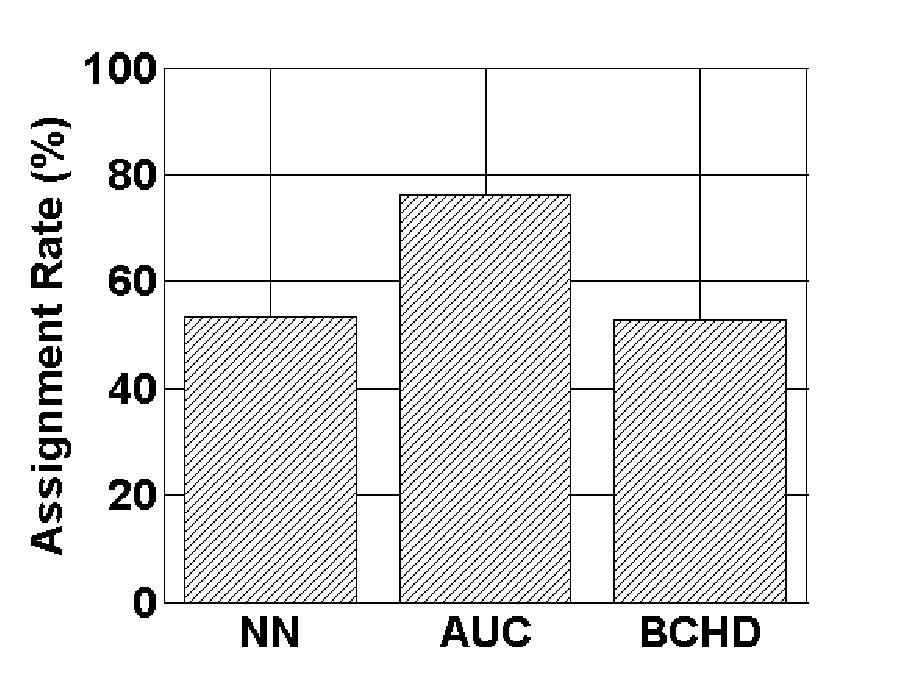
\includegraphics[width = 0.30\columnwidth]{figures/gowalla.eps}
    }
    \subfigure[Foursquare]{
        \label{fig:foursquare}
        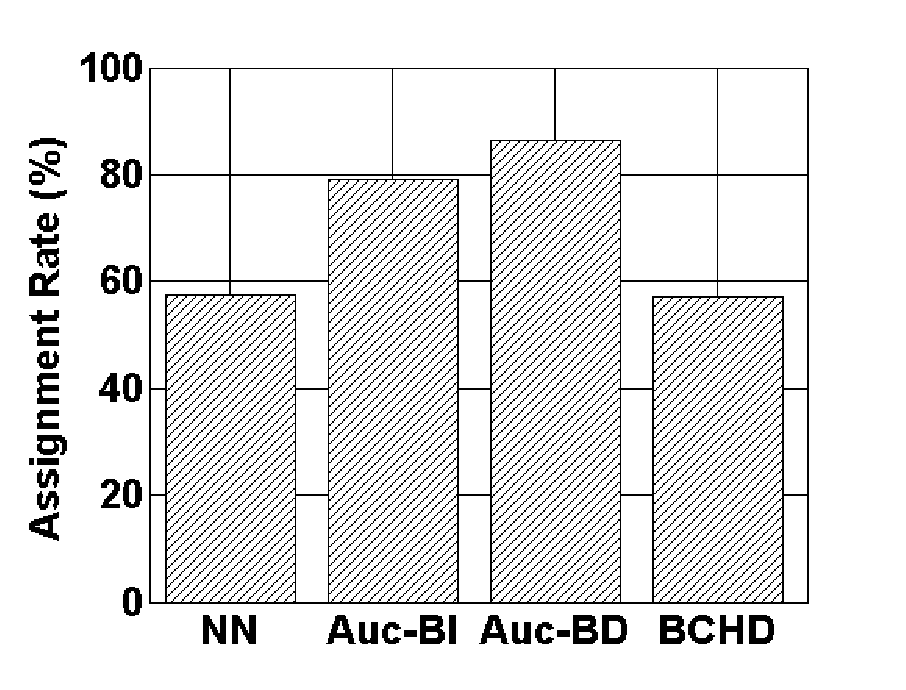
\includegraphics[width = 0.30\columnwidth]{figures/foursquare.eps}
    }
    \subfigure[Synthetic]{
        \label{fig:syn}
        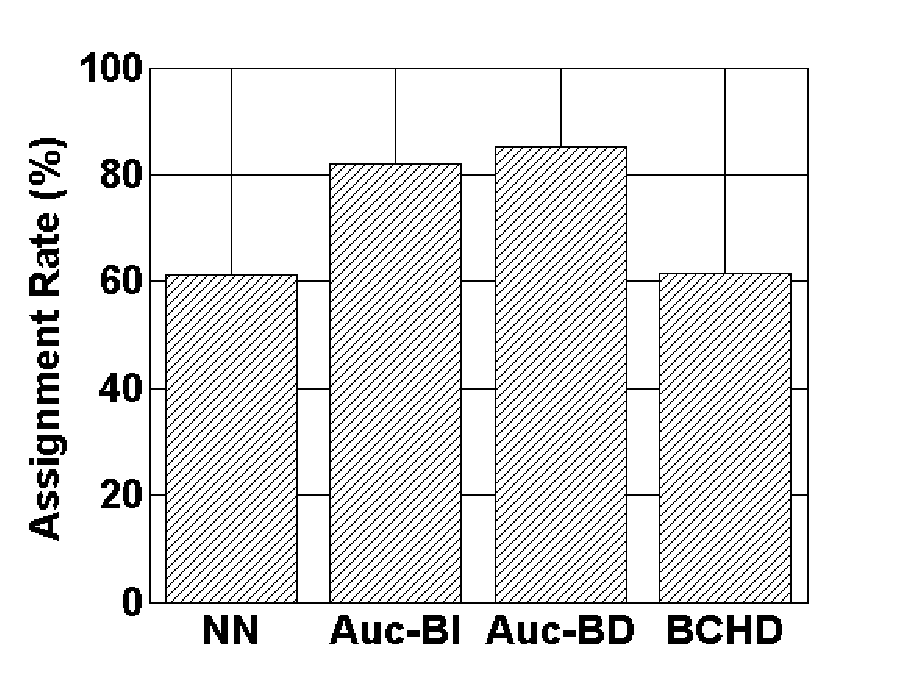
\includegraphics[width = 0.30\columnwidth]{figures/syn.eps}
    }
    \vspace{-0.15in}
    \caption{Assignment Rate of Real-Time Approaches}
    \label{fig:quality}
\end{figure}

First we compare the assignment rate of different algorithms. \cref{fig:quality} depicts that AUC outperform NN by almost 25\%. The main reason is that AUC performs the scheduling and matching phases in tandem. However, NN is an SOM approach where the schedule of the worker is not considered when a task is matched with him. Consequently, it is likely that a task gets assigned to a worker while the worker is not able to schedule it and thus, the task does not get completed. Furthermore, AUC outperform BCHD by almost a similar margin. This is because BCHD performs the matching phase, the schedule of the worker is not considered and hence, a task might end up getting matched to and scheduled for a worker that was not the best worker. This in turn can lower the chances of that worker to get assigned to a new task in the future. The second reason is that while a task is waiting at the server to get processed with the next batch, depending on the length of the batching  interval, it will lose some portion of its available time before its deadline, which in turn, can lower the chances of the task fitting a worker's schedule (more details in \cref{subsec:exp_scale}).

\begin{figure}[h]
    \centering
    \subfigure[NN]{
        \label{fig:nn_comp}
        \includegraphics[width = 0.30\columnwidth]{figures/nn.eps}
    }
    \subfigure[AUC]{
        \label{fig:bi_comp}
        \includegraphics[width = 0.30\columnwidth]{figures/bi.eps}
    }
    \subfigure[BCHD]{
        \label{fig:bchd_comp}
        \includegraphics[width = 0.30\columnwidth]{figures/bchd.eps}
    }
    \vspace{-0.15in}
    \caption{\small{Assignment Profile-Varying Worker/Task Arrival Rates}}
    \label{fig:tw_rate}
\end{figure}

In order to study the effect of temporal parameters of SC, we ran several experiments using different pairs of task arrival rates ($t_{rate}$) and worker arrival rates ($w_{rate}$). \cref{fig:tw_rate} illustrates the effect of increasing $t_{rate}$ and $w_{rate}$ on the assignment rate. The level of grayness corresponds to the percentage of completed tasks with black and white representing 100\% and 0\%, respectively. With small number of workers, as$t_{rate}$ increases, the percentage of completed tasks decreases where at the top left corner of each plot we get close to 0\%. On the other hand with small number of incoming tasks, as we increase $w_{rate}$, eventually all tasks will be completed.

\begin{figure}[h]
	\centering
    \subfigure[Auc-BI Vs. NN]{
        \label{fig:bi_nn}
        \includegraphics[width = 0.30\columnwidth]{figures/bi_nn.eps}
    }
    \subfigure[Auc-BI Vs. BCHD]{
        \label{fig:bi_bchd}
        \includegraphics[width = 0.30\columnwidth]{figures/bi_bchd.eps}
    }
    \subfigure[AUC Vs. ApproxAUC] {
		\label{fig:bi_abi}
		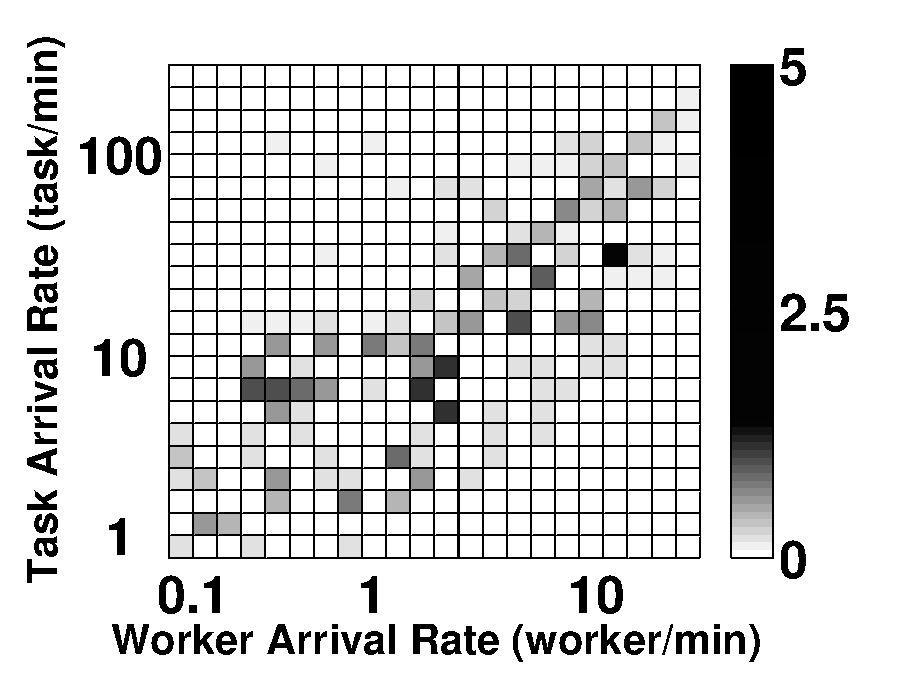
\includegraphics[width = 0.30\columnwidth]{figures/bi_abi.eps}	    
    }
    \vspace{-0.15in}
	\caption{Pairwise Difference in Assignment Rates}
\end{figure}

To better evaluate the difference between alternative algorithms, in \cref{fig:bi_nn,fig:bi_bchd} we performed a pair-wise comparison of different algorithms by taking their task completion rates. For example, \cref{fig:bi_nn} shows the difference between AUC and NN. We observe that all approaches perform similarly at the two extreme cases discussed in \cref{fig:tw_rate}, i.e., high task-low worker and low task-high worker. AUC outperforms NN and BCHD up to 30\% when the problem is more complex, i.e., outside the extreme cases. An interesting observation in \cref{fig:bi_nn} is that AUC outperforms NN by a larger margin at scale (higher $t_{rate}$ and $w_{rate}$). The reason is that with higher $t_{rate}$ and $w_{rate}$ more workers are moving around and more tasks arrive and leave so in general the spatiotemporal dynamism of the system increases. AUC takes advantage of the dynamism by guaranteeing a task gets assigned to a worker that can complete it. On the contrary, NN ignores the schedule of a worker during matching and this becomes more important as there is more dynamism in the system.

We mentioned earlier that with Auction-SC, the workers perform an exhaustive search to find out if they can fit a new task into their schedule (\cref{algo:can_schedule}). As workers accept new tasks, they also complete some other tasks so as we observed in our experiments, performing an exhaustive search did not cause any scalability issues. Nevertheless, one might want to replace the exhaustive search with a polynomial time approximate algorithm. With ApproxBI, we use the insertion algorithm from \cite{Rosenkrantz74} that runs in $O(n^2)$. \cref{fig:bi_abi} depicts the change affects the assignment rate by less than only 5\%.
%The difference caused by ApproxBI is that the workers that are eligible for a task using Auc-BI, may not be able to fit the task in their schedules using ApproxBI due to the approximation. As a result, using ApproxBI the server may not be able to assign some tasks even if they can be completed using Auc-BI. Fortunately, as shown in \cref{fig:bi_abi}, that does not happen very often regardless of $t_{rate}$ and $w_{rate}$.

%The next set of experiments compare the effect of the spatial distribution of tasks. We compared the quality of the final assignment for three different distributions. Even though real-world data usually follow a skewed spatial distribution (\cref{subsec:dataset}), the results of these experiments show that regardless of the distribution, Auc-BI and Auc-BD outperform NN and BCHD. With the first distribution, the location of the tasks follow a spatial Poisson process \cite{Baddeley07}. The other two distributions are a Uniform 2D distribution and a Skewed distribution. The results in \cref{fig:dists} show that Auc-BI and Auc-BD generate assignments at least 20\% better than NN and BCHD. Also, we can see with Poisson and Uniform distributions, there is not much difference between Auc-BI and Auc-BD. The reason is that both distributions generate tasks at completely random locations. Consequently, tasks are released at every area with the same probability and hence Auc-BD does not have any advantage over Auc-BI.

%\begin{figure}[h]
%	\centering
%	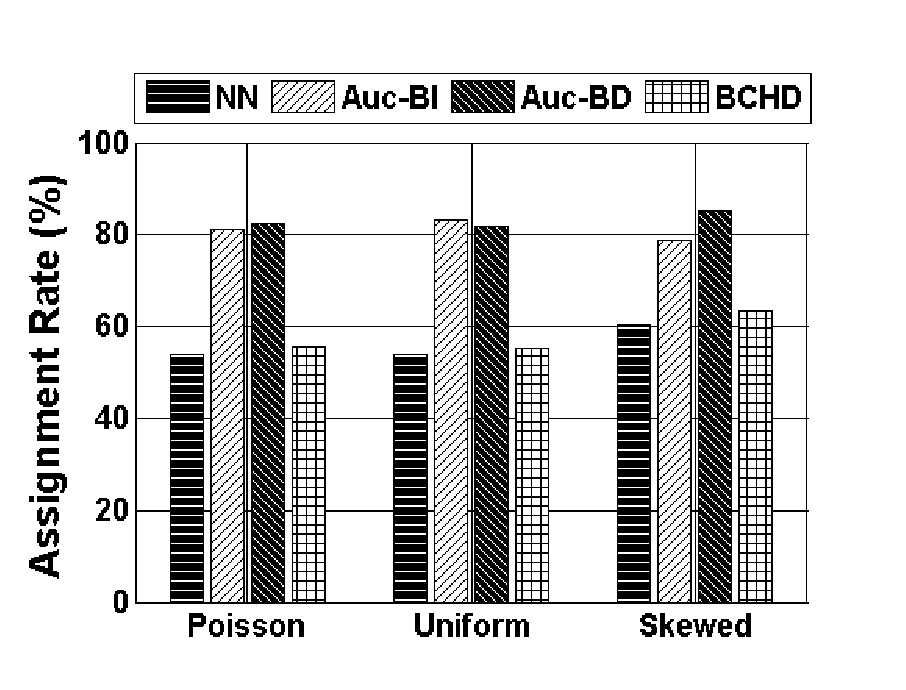
\includegraphics[width=0.30\columnwidth]{figures/dists.eps}
%	\vspace{-0.1in}
%	\caption{Assignment Difference-Varying Distribution}\label{fig:dists}
%\end{figure}
\vspace{-0.05in}
\subsection{Scalability}
\label{subsec:exp_scale}
\vspace{-0.05in}
The last set of experiments focus on comparing the scalability of AUC with BCHD and MONO. We can measure the scalability of a SC systems by the average time required to process a task which in turn indicates the throughput of the system. \cref{fig:runtime} illustrates the average processing time of a single task in different algorithms for different worker arrival rates. As shown in \cref{fig:runtime}, as the arrival rate of workers increases, the average processing time of a single task in AUC does not change since AUC utilizes the workers for scheduling an incoming task. On the contrary, with MONO and BCHD, in addition to performing matching, the server also performs scheduling for all the workers. Consequently, with these algorithms, the average processing time of a single task grows as we increase the number of workers and is several orders of magnitude higher than that of AUC.

\begin{figure}[h]
    \centering
    \subfigure[MONO]{
        \label{fig:runtime_mbi}
        \includegraphics[width = 0.30\columnwidth]{figures/run_time_mbi.eps}
    }
    \subfigure[AUC]{
        \label{fig:runtime_abi}
        \includegraphics[width = 0.30\columnwidth]{figures/run_time_abi.eps}
    }
    \subfigure[BCHD]{
        \label{fig:runtime_bchd}
        \includegraphics[width = 0.30\columnwidth]{figures/run_time_bchd.eps}
    }
    \vspace{-0.15in}
    \caption{Average processing time for a single task}
    \label{fig:runtime}
\end{figure}

The next set of experiments, compares the \emph{queuing delay} of tasks as the duration between the time the task arrives at the server and the time the server starts processing it. \cref{fig:queue} compares the average queuing delay of tasks for AUC and MONO after running them for 1 hour (because BCHD does not process tasks one at a time, the concept of queuing delay is different). As depicted in \cref{fig:queue}, MONO suffers from queuing delays with less than 10 tasks/second. On the other hand, with AUC we do not observe queuing delays for up to 50 tasks/second.

\begin{figure}[h]
	\centering
	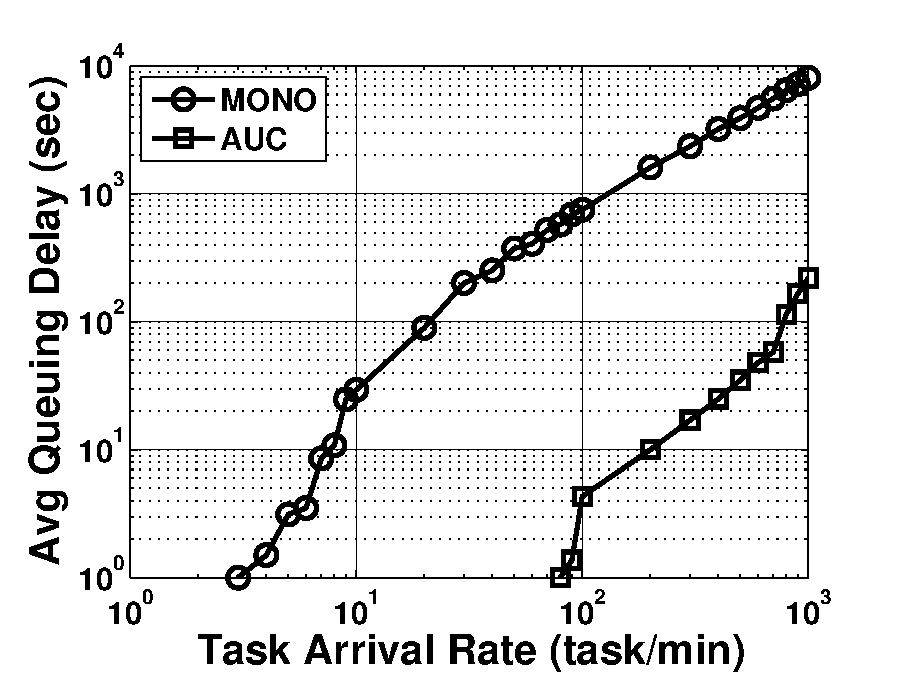
\includegraphics[width = 0.4\columnwidth]{figures/queue.eps}
	\vspace{-0.1in}
	\caption{Average queuing delay}\label{fig:queue}
\end{figure}

Earlier we explained that with BCHD, a task has to wait in a queue for the server to finish processing the previous batch. Depending on the batching interval, the negative effect of batching can propagate over time. For example, assuming $t_{rate} = 10$ tasks/sec, if we start with a batching interval of 1 second, the first batch will run with \textasciitilde 10 tasks. If processing the first batch takes 2 seconds, by the time we want to process the second batch \textasciitilde 20 tasks have been queued and have to be processed. Consequently, the second batch will take longer than 2 seconds and so on and so forth. In \cref{fig:bs} we run BCHD with a $t_{rate} = 10$ tasks/sec. We measure the following three metrics for different batches over time: (1) the number of tasks per batch, (2) the processing time of each batch and (3) the average queuing delay of tasks in each batch. \cref{fig:bs} depicts how the negative effects of batching propagates over time.

\begin{figure}[h]
    \centering
    \subfigure[Tasks per Batch]{
        \label{fig:bs_tpb}
        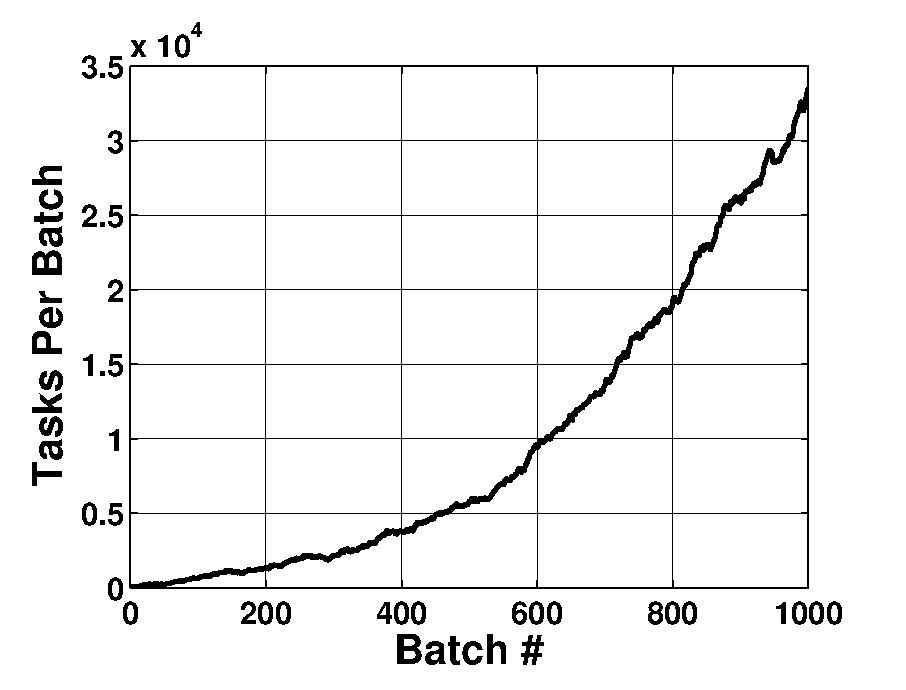
\includegraphics[width = 0.3\columnwidth]{figures/bs_tpb.eps}
    }
    \subfigure[Batch Processing Time]{
        \label{fig:bs_bpt}
        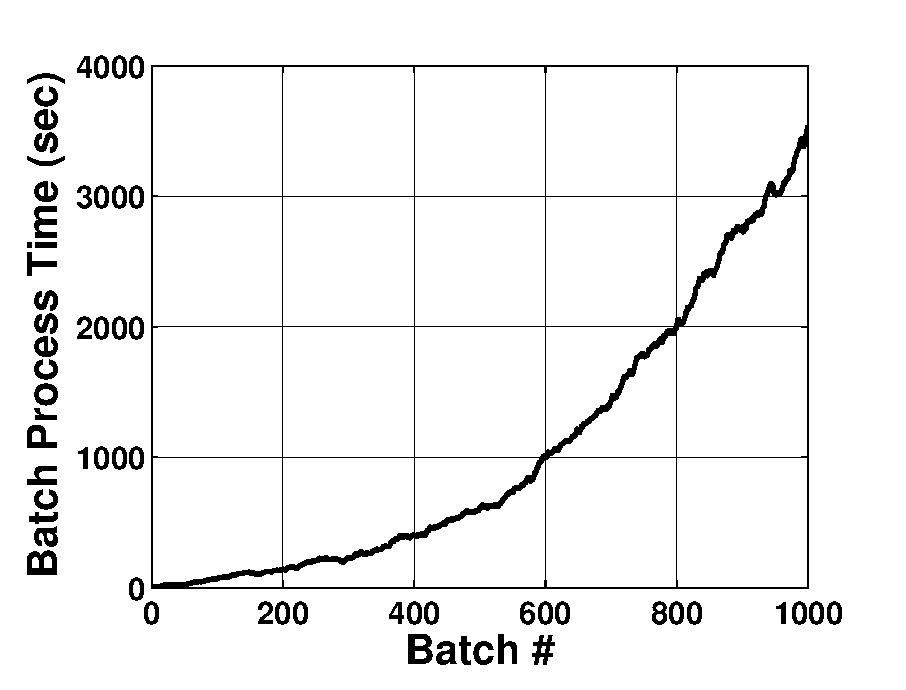
\includegraphics[width = 0.3\columnwidth]{figures/bs_bpt.eps}
    }
    \subfigure[Task Avg Delay per Batch]{
        \label{fig:bs_tad}
        \includegraphics[width = 0.3\columnwidth]{figures/bs_tad.eps}
    }
    \vspace{-0.15in}
    \caption{BCHD Scalability ($tRate = 10 task/minute$)}
    \label{fig:bs}
\end{figure}

%\cref{fig:bss} shows the same three metrics when varying the task arrival rate. As it can be seen, for $t_{rate} < 10$ tasks/sec, the processing time of each batch does not change over time. However, for a task arrival rate of only 10 tasks/second, BCHD can no longer scale.

%\begin{figure}[h]
%   \centering
%    \subfigure[Tasks per Batch]{
%        \label{fig:bs_tpb}
%        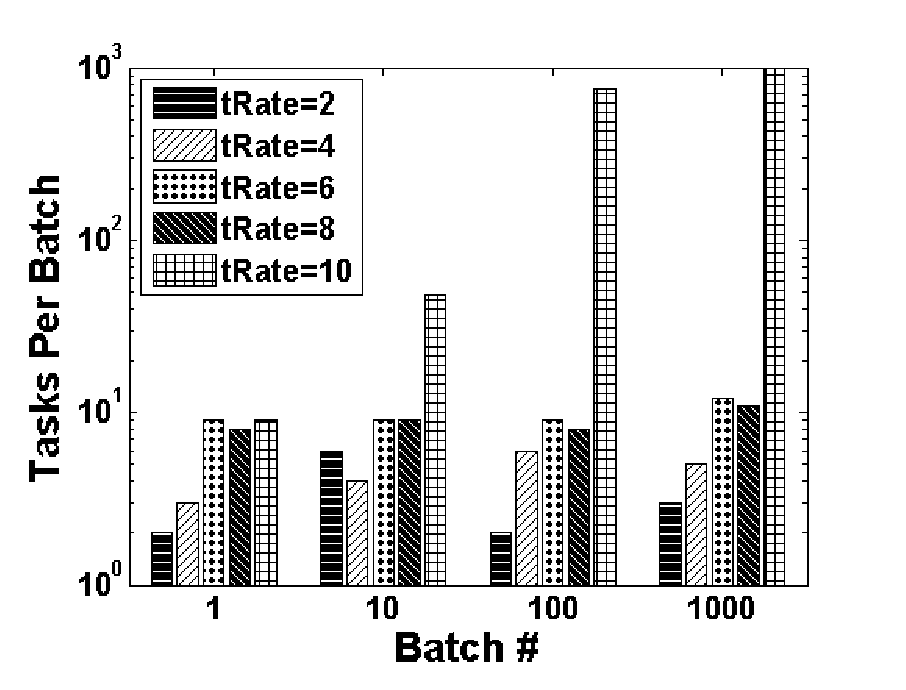
\includegraphics[width = 0.45\columnwidth]{figures/bss_tpb.eps}
%    }
%    \subfigure[Batch Processing Time]{
%        \label{fig:bs_bpt}
%        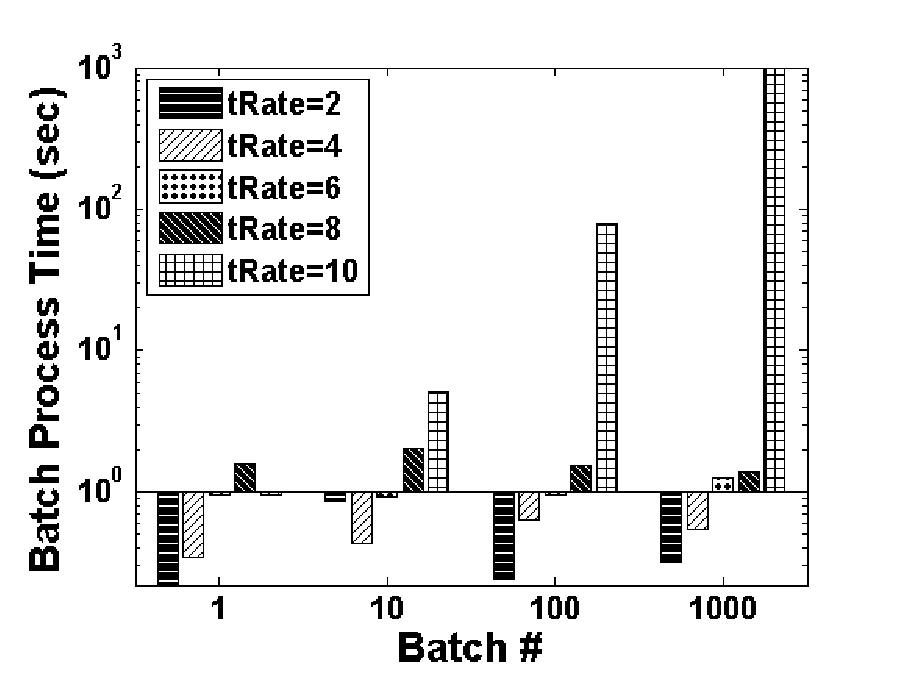
\includegraphics[width = 0.45\columnwidth]{figures/bss_bpt.eps}
%    }
%    \subfigure[Task Avg Delay per Batch]{
%        \label{fig:bs_tad}
%        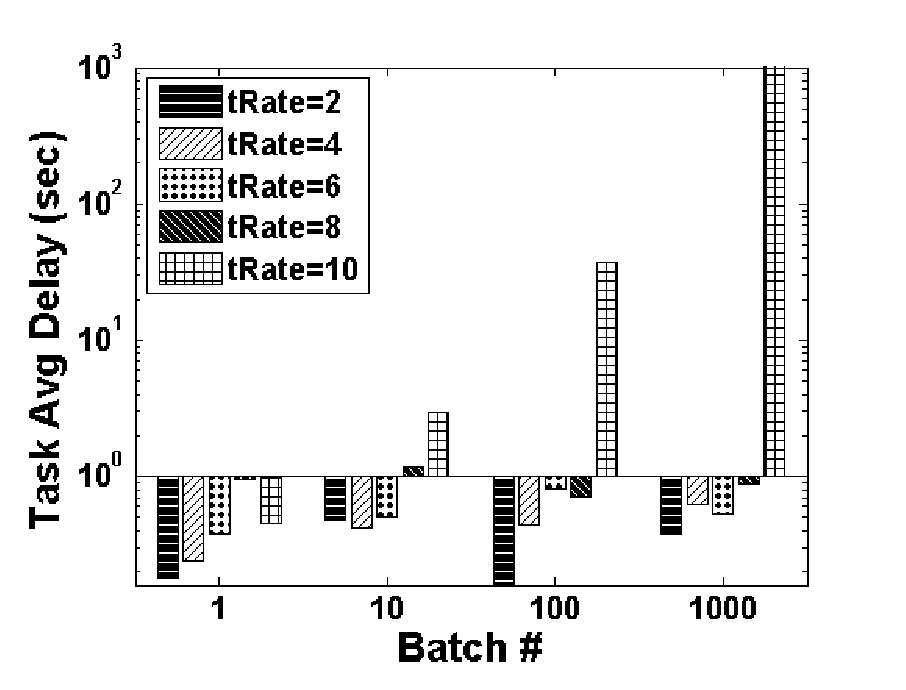
\includegraphics[width = 0.45\columnwidth]{figures/bss_tad.eps}
%    }
%    \vspace{-0.15in}
%    \caption{BCHD Scalability}
%    \label{fig:bss}
%\end{figure}

To provide a more practical perspective, in \cref{fig:req} we compare the scalability of different approaches given the current minimum requirements of a ride sharing application in New York City \cite{NYCTaxi}. As shown, while MONO and BCHD cannot satisfy the current requirements, AUC can scale much higher than what currently is needed.

\begin{figure}[h]
	\centering
	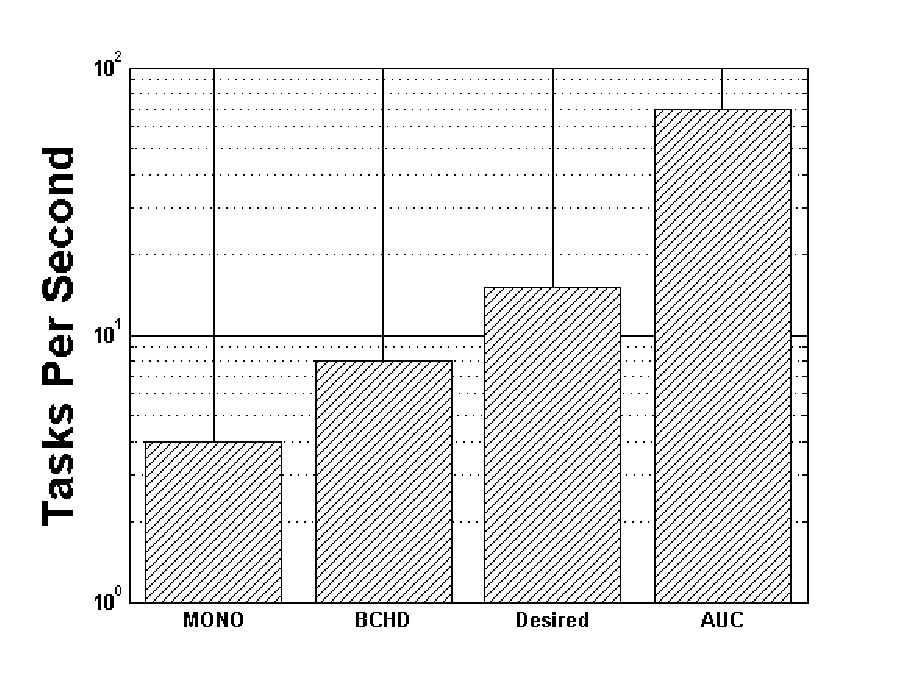
\includegraphics[width = 0.3\columnwidth]{figures/scale_req.eps}
	\vspace{-0.1in}
	\caption{Real-world Scalability Requirements}\label{fig:req}
\end{figure}

To summarize the results of our experiments, we showed that SOM approaches cannot generate high assignment rates since they do not consider the schedule of workers when assigning tasks. With batched approaches, tasks are not necessarily assigned to the best workers and long batching intervals reduce the chance of new tasks fitting in a workers schedule. On the other hand, the immediate assignment of tasks along with consideration of scheduling at the time a task is being matched are the main reasons for the better overall assignment rate of Auction-SC algorithms. Furthermore, because of the costly many-to-many matching, batched approaches cannot scale. Even with an online monolithic-SC server where tasks are processed one at a time, the server has to perform scheduling for all workers. Performing scheduling for large number of workers is time consuming and prevents online monolithic-SC approaches from scaling. However, with Auction-SC, tasks are processed one at a time (i.e., fast matching) and the server utilizes the workers for performing scheduling (i.e., fast scheduling).
%\cref{tab:summary} shows the summary of our experimental results.

%\begin{table*}
%  \centering
%  \begin{tabular}{|c|c|c|c|c|c|c|c|c|}
%    \hline
%    \multicolumn{2}{|>{\columncolor{kugray5}}c|}{}&\multicolumn{4}{c|}{non-SC bidding rules}&\multicolumn{2}{c|}{SC bidding rules}\\
%    \arrayrulecolor{kugray5}
%    \arrayrulecolor{black}
%    \cline{3-8}
%    \multicolumn{2}{|>{\columncolor{kugray5}}c|}{}&Rnd&Rnk&NN&MFT&BI&BD\\
%    \hline
%    \multirow{2}{*}{Centralized}&Scalability&Bad&Bad&Bad&Bad&Very Bad&Very Bad\\
%    \cline{2-8}
%                         		&Assignment Quality&Very Bad&Very Bad&Bad&Very Bad&Very Good&Very Good\\
%    \hline
%    \multirow{2}{*}{Auction-SC}&Scalability&Very Good&Very Good&Very Good&Very Good&Good&Good\\
%    \cline{2-8}
%                         		&Assignment Quality&Very Bad&Very Bad&Bad&Very Bad&Very Good&Very Good\\
%    \hline
%  \end{tabular}
%  \vspace{-0.1in}
%  \caption{Summary of Experimental Results}
%  \label{tab:summary}
%\end{table*}